%!TEX root = Presentation-Thoma.tex
\section{Problemstellung}
\subsection{Problemstellung}

\begin{frame}{Problemstellung}
    \begin{figure}[ht]
        \begin{minipage}[b]{0.45\linewidth}
            \centering
            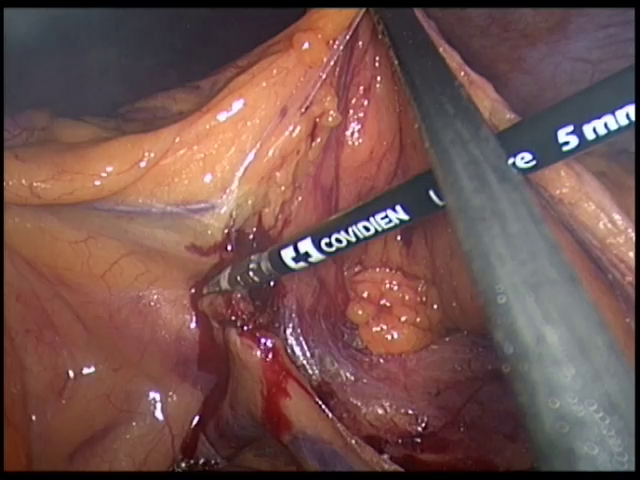
\includegraphics[width=\textwidth]{../images/img_19_raw.png}
            \caption{Endoskop-Bild (input)\newline RGB-Bilder mit $\SI{640}{\px} \times \SI{480}{\px}$ als Eingabe.}
            \label{fig:semantic-segmentation-input}
        \end{minipage}
        \hspace{0.5cm}
        \begin{minipage}[b]{0.45\linewidth}
            \centering
            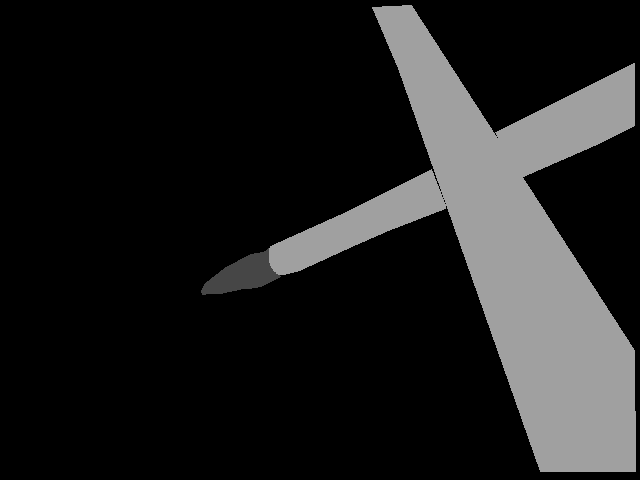
\includegraphics[width=\textwidth]{../images/img_19_class.png}
            \caption{Segmentation mask (output)\newline 3-Farben Bilder mit $\SI{640}{\px} \times \SI{480}{\px}$ als Segmentierungsmaske}
            \label{fig:semantic-segmentation-output}
        \end{minipage}
    \end{figure}


    Die Daten stammen aus Endoscopic Sub-Challenge
              \enquote{Instrument Segmentation and Tracking}.
\end{frame}

\begin{frame}{Taxonomie nach Thoma 2016: A survey of semantic segmenation}
    \begin{itemize}
        \item Klassen: (1) Medizinisches Instrument (2) Nicht \enquote{medizinisches Instrument} / Hintergrund
        \item Jeder Pixel gehört zu genau einer Klasse.
        \item Daten: vgl. vorherige Folie
        \item Keine Tiefeninformationen; keine Stereo-Bilder; 2D
        \item Passive, automatische Segmentierung
    \end{itemize}
\end{frame}
